\documentclass[letterpaper]{article}
\usepackage{aaai2026}
\usepackage{times}
\usepackage{helvet}
\usepackage{courier}
\usepackage[hyphens]{url}
\usepackage{graphicx}
\urlstyle{rm}
\def\UrlFont{\rm}
\usepackage{natbib}
\usepackage{caption}
\usepackage{amsmath,amssymb}
\frenchspacing
\setlength{\pdfpagewidth}{8.5in}
\setlength{\pdfpageheight}{11in}
\pdfinfo{
/TemplateVersion (2026.1)
}

\setcounter{secnumdepth}{0}

\title{Active Data Acquisition with Side Information via Discrete Diffusion Priors}

\author{
    An Vuong\textsuperscript{\rm 1},
    Anthony Q. Nguyen\textsuperscript{\rm 2},
    Thuan Nguyen\textsuperscript{\rm 2},
    Thinh Nguyen\textsuperscript{\rm 1}
}
\affiliations{
    \textsuperscript{\rm 1}School of Electrical Engineering and Computer Science, Oregon State University, Corvallis, OR 97331\\
    \textsuperscript{\rm 2}Department of Engineering, East Tennessee State University, Johnson City, TN 37614\\
    \{vuonga2, thinhq\}@oregonstate.edu, anth.nguyen2357@gmail.com, nguyent11@etsu.edu
}

\begin{document}
\maketitle

\begin{abstract}
Modern learning systems depend on high-fidelity data, yet acquisition is costly: higher measurement fidelity increases power, storage, and the risk of collecting irrelevant content, while aggressive cost reduction can discard information critical to downstream analysis. We address this cost--fidelity trade-off with an information-theoretic framework that balances \emph{specificity} and \emph{generality}---acquiring data maximally relevant to a broad set of tasks without tying acquisition to any particular classifier. Mutual information serves as a model-agnostic relevance metric. We formulate budgeted pixel selection as Problem P4: choose a mask distribution $p(x \mid z)$, conditioned on side information $z$, to maximize $I(Y; C)$ between a target discrete image $C$ and a partial observation $Y$, subject to sparsity constraints on the sensing action $X$. Because $H(C)$ is independent of the mask, this is equivalent to minimizing $H(C \mid Y)$. The acquisition problem is inherently hard in high dimensions; when $p(y \mid x, c)$ is unknown, we approximate it with a \textbf{frozen Discrete Denoising Diffusion Probabilistic Model (D3PM)} that supplies a differentiable conditional-entropy surrogate. A spatial mask network implements $p_\phi(x \mid z)$ with masked-only entropy, empirical sparsity--timestep calibration, and Gumbel-Softmax relaxation. On MNIST, the proxy $H(C \mid Y)$ decreases from $0.029$ to $0.006$ over 40 epochs while respecting sparsity budgets. We then stress-test the framework on a real inverse problem---Cartesian phase-encode selection for accelerated MRI on fastMRI---where the proxy can be scored against reconstruction error rather than against itself. \textbf{The framework does not survive that test in its conditional form.} Under a budget-exact, held-out protocol, the entropy proxy disagrees with reconstruction quality; conditioning the mask on per-slice side information is worth at most $2\%$ and only at the tightest budget; and a $300$-number average of per-row k-space energy outperforms the learned policy. What does work is optimising the \emph{discrete} mask directly against a reconstructor: a learned static mask beats variable-density sampling by $1.5$--$3.8\%$ NMSE under a reconstructor it never saw during optimisation. We report the negative results, the controls that establish them, and a metric defect that inverted two of our own earlier conclusions, and release the modular \texttt{itw/} package.
\end{abstract}

\noindent\textbf{Keywords:} Entropy; mutual information; active sensing; discrete diffusion; side information.

\section{Introduction}

Modern data science increasingly relies on analyzing large volumes of data---often, the more data, the better. However, the \emph{quality} of the data is heavily influenced by how it is acquired. Accurate, comprehensive sensing can yield high-fidelity measurements, but at the cost of increased power consumption, bandwidth, storage, and processing time, and may also raise the risk of collecting information irrelevant to the target application. Conversely, reducing acquisition cost can lower fidelity and cause loss of information crucial to downstream tasks such as classification, segmentation, or generative modeling.

Consider \textbf{budgeted pixel sensing}. In medical imaging, remote sensing, bandwidth-limited transmission, or interactive annotation, only a fraction of pixels may be measured or labeled. The design question is not merely \emph{how many} pixels to observe, but \emph{which} locations carry the most information about the full scene under a fixed budget---analogous to optimizing radar transmit parameters to target effective frequency ranges while avoiding unnecessary power use. A highly task-specific policy can produce an overly specialized dataset that excludes information needed for related tasks. Ideally, we collect data rich and versatile enough to support not only the immediate task but similar, yet unspecified, ones.

We adopt an \textbf{information-theoretic perspective} that balances specificity and generality. Rather than optimizing acquisition solely to improve one learning algorithm, we seek measurements whose relevance is measured by \textbf{mutual information}---a robust, model-agnostic quantity not tied to a particular hypothesis class \cite{cover2006elements}. As illustrated in Figure~\ref{fig:pipeline}, we select a sensing action $X$ (a binary pixel mask) based on \textbf{side information} $Z$---class label, a coarse image summary, and a sparsity target---to produce a measurement $Y$ that shares maximal information with the target $C$.

In prior work \cite{vuong2025cnc}, we showed that when probabilistic acquisition models are unknown, deep networks can learn effective masks by combining a U-Net generator \cite{ronneberger2015unet} with \textbf{MINE} \cite{belghazi2018mine} to estimate $I(Y; C)$ on continuous CelebA images \cite{liu2015celeba}. \textbf{This paper} extends that line to \textbf{discrete} images and replaces the separate MI estimator with a \textbf{frozen absorbing-state D3PM} \cite{austin2021structured} as a conditional-entropy proxy for $H(C \mid Y)$, coupled with masked-only aggregation, empirical calibration between mask density and diffusion timestep, and Gumbel-Softmax training. The D3PM weights remain fixed; only the mask generator is updated.

\subsection{Contributions}
\begin{itemize}
\item We cast active data acquisition with side information as \textbf{Problem P4}---maximizing $I(Y; C)$ under sparsity constraints---and implement it for discrete images via minimization of a D3PM-based $H(C \mid Y)$ proxy.
\item We introduce \textbf{masked-only entropy}, restricting the proxy to observed pixels so gradients target informative locations rather than trivial absorbed regions.
\item We propose \textbf{empirical sparsity--timestep calibration} mapping mask density to D3PM noise level via pixel survival under the forward absorbing process.
\item We \textbf{stress-test the framework on accelerated MRI}, where masks can be scored by reconstruction error rather than by the proxy that selected them, and report three negative results: the entropy proxy anti-correlates with reconstruction quality at the tightest budget; instance-adaptive conditioning does not pay; and a $300$-parameter energy average beats the learned policy under zero-filled reconstruction.
\item We show that \textbf{mask ranking is reconstructor-dependent}---the energy-optimal mask is the best of all under zero-filled reconstruction and the worst once a learned prior exists---which explains the failure and dictates what a sampling objective must be trained against.
\item We contribute an \textbf{evaluation protocol and two controls} that this literature does not routinely apply: a scout-derangement test that isolates whether conditioning is used at all, and a held-out \emph{judge} reconstructor that separates genuine mask quality from overfitting to the reconstructor used during optimisation (worth up to $1.5$ pp here).
\item We release a modular \texttt{itw/} package with spatial and row mask architectures, a reconstructor, budget-exact seeded evaluation, and Jupyter workflows for MNIST and CIFAR-10.
\end{itemize}

\section{Related Work}

\paragraph{Target detection and radar.}
Object identification via radar and related sensors has been studied extensively with model-driven methods \cite{kay1998detection} and data-driven detectors \cite{han2021radar}. Unlike these approaches, we optimize the \textbf{information content} of acquired measurements for downstream use under resource constraints.

\paragraph{Learned sampling for MRI.}
Variable-density random sampling with a fully sampled low-frequency block is the standard heuristic for Cartesian compressed-sensing MRI \cite{lustig2007sparse}. Learning the pattern instead has two established lines: \emph{combinatorial} selection, where masks are built greedily to minimize reconstruction error on a training set \cite{gozcu2018learning}, and \emph{relaxation-based} selection, where a differentiable probabilistic mask is trained jointly with a reconstruction network \cite{bahadir2020loupe}. \textbf{We claim neither as novel}; our MRI experiments deliberately re-derive both in order to test whether an information-theoretic, instance-adaptive policy improves on them. It does not, and our strongest MRI result is obtained by the combinatorial route. What we add is the diagnosis of \emph{why} the information-theoretic route fails, and the controls that establish it.

\paragraph{Active learning.}
Active learning selects informative samples for labeling to improve a particular model \cite{guo2007active}. Most methods are tailored to a classifier. We instead maximize mutual information, decoupling acquisition from any single learning algorithm. \citet{shayovitz2023universal} minimize conditional information in a universal active-learning framework; our emphasis is \textbf{spatial acquisition masks} under explicit pixel budgets.

\paragraph{Prior ITW acquisition work.}
\citet{vuong2025cnc} formulate Problems P1--P4 for active acquisition with side information and propose MINE-based blind estimation with U-Net masks on CelebA, where masks emphasize high-frequency structure. We inherit the P4 formulation and side-information architecture but move to discrete state spaces and a D3PM prior.

\paragraph{Discrete diffusion.}
D3PMs \cite{austin2021structured} extend denoising diffusion to categorical data via structured transition matrices, including absorbing-state kernels aligned with masked prediction. Our codebase implements absorbing-state D3PM with cosine $\beta$ scheduling in PyTorch \cite{ryu2024d3pm}.

\paragraph{Continuous diffusion.}
DDPMs \cite{ho2020ddpm} underpin much of generative modeling; DiT \cite{peebles2023dit} replaces U-Nets with transformers and serves as the CIFAR-10 backbone. Our setting requires \textbf{discrete} states and explicit mask tokens.

\paragraph{Differentiable discrete masks.}
Gumbel-Softmax \cite{jang2017gumbel,maddison2017concrete} enables gradient-based learning over binary structures via relaxation and straight-through estimation.

\paragraph{Information-theoretic diffusion.}
Recent work relates denoising objectives to information quantities in masked diffusion \cite{nie2025lld}. Our proxy is simpler---sum of per-pixel categorical entropies from a frozen $c_0$-predictor---but points toward tighter variational bounds as future work.

\section{Problem Description}

\subsection{Notation}
\begin{table}[t]
\centering
\footnotesize
\begin{tabular}{@{}p{0.28\columnwidth}p{0.62\columnwidth}@{}}
\hline
\textbf{Symbol} & \textbf{Description} \\
\hline
$C$, $p(c)$ & Target discrete image and its distribution \\
$X$, $p(x \mid z)$ & Sensing action (binary mask) and conditional distribution \\
$Y$, $p(y \mid x, c)$ & Measurement (partial observation) and distribution \\
$Z$, $p(z \mid c)$ & Side information (label, coarse image, sparsity budget) \\
\hline
\end{tabular}
\caption{Notation for active data acquisition with side information.}
\label{tab:notation}
\end{table}

An active data acquisition model with side information is specified by $p(c)$, $p(z \mid c)$, and $p(y \mid x, c)$. We parameterize $p(x \mid z)$ with a neural network $p_\phi(x \mid z)$ rather than enumerating extreme points of the probability simplex \cite{vuong2025cnc}.

\subsection{Acquisition Model}
Images are discretized to $N$ bins per channel: $C \in \{0,\ldots,N-1\}^{C_{\mathrm{ch}} \times H \times W}$. A mask $X \in [0,1]^{1 \times H \times W}$ (binary at inference) selects observed pixels:
\begin{equation}
Y = f(C, X),
\end{equation}
where $f$ sets unobserved locations to absorbing state $0$. For binary MNIST ($N{=}2$), $f(C,X) = X \odot C$. For multi-channel CIFAR ($N{=}8$), observed bins are remapped to $\{1,\ldots,N-1\}$ so that $0$ exclusively denotes ``masked.''

Side information $Z$ comprises the class label $c$, an $8 \times 8$ grayscale summary of $C$, and a target sparsity $s = \mathbb{E}[X]$ drawn per batch from $\mathcal{U}(s_{\min}, s_{\max})$.

\subsection{Problem P4 and Equivalence}
With side information, the primary formulation is:
\begin{equation}
\max_{p(x \mid z)} \; I(Y; C) \quad \text{subject to} \quad g_i\bigl(p(x \mid z)\bigr) \le 0.
\label{eq:p4}
\end{equation}
Related problems P1--P3 maximize $I(X,Y;C)$ or $I(Y;C)$ without conditioning on $Z$ \cite{vuong2025cnc}. We focus on \textbf{P4} because the mask policy should adapt to available context. A typical cost constraint is expected sparsity: $\mathbb{E}[\sum_i X_i] = s \cdot HW$, enforced via $\mathcal{L}_{\mathrm{sparsity}} = \mathbb{E}[(\bar{X} - s)^2]$.

Since $I(Y; C) = H(C) - H(C \mid Y)$ and $H(C)$ does not depend on $X$, maximizing mutual information is equivalent to minimizing $H(C \mid Y)$.

\subsection{Computational Challenge}
\citet{vuong2025cnc} show that optimal solutions to P1--P4 lie at extreme points of convex feasible regions; enumerating them is NP-hard in high dimensions. When acquisition models are \textbf{known}, iterative methods such as CCCP can approximate solutions. For image masking, we use parametric $p_\phi(x \mid z)$ and a differentiable surrogate for $H(C \mid Y)$ (Section~\ref{sec:blind}).

\section{Neural Blind Estimation}
\label{sec:blind}

\subsection{When Models Are Unknown}
When $p(y \mid x, c)$ is unavailable, \citet{vuong2025cnc} train networks for $p(x \mid z)$ and $I(Y; C)$ (MINE), with $Y = X \odot C$ and $Z = G * C$ (Gaussian blur). Sparsity is encouraged via a logarithmic mask penalty combined with $\mathcal{L}_{\mathrm{MINE}}$. On CelebA, learned masks emphasize high-frequency regions; Fourier-domain experiments confirm preference for high-frequency components. MINE can exhibit high variance, and continuous formulations do not directly apply to quantized discrete images.

\subsection{D3PM Conditional-Entropy Proxy}
We replace MINE with a \textbf{frozen} pretrained D3PM modeling $p(C)$ and supplying per-pixel predictive uncertainty. A D3PM defines forward transitions $q(c_t \mid c_{t-1})$ and a denoiser $p_\theta(c_0 \mid c_t, t, c_{\mathrm{lbl}})$.

\begin{table}[t]
\centering
\footnotesize
\begin{tabular}{@{}p{0.22\columnwidth}p{0.32\columnwidth}p{0.32\columnwidth}@{}}
\hline
\textbf{Component} & \textbf{MNIST} & \textbf{CIFAR-10} \\
\hline
Backbone & DummyX0Model & DiT\_Llama ($d{=}1024$) \\
Classes $N$ & 2 & 8 \\
Steps $T$ & 1000 & 1000 \\
Schedule & Cosine $\beta$ & Cosine $\beta$ \\
Checkpoint & absorb\_cosine\_399 & absorb\_cosine\_499 \\
\hline
\end{tabular}
\caption{Frozen D3PM priors used for mask training.}
\label{tab:d3pm}
\end{table}

All D3PM parameters are frozen during mask training. Given $Y$, timestep $t$, and label $c_{\mathrm{lbl}}$, per-pixel Shannon entropy is:
\begin{equation}
H_i = -\sum_{k=0}^{N-1} p_i(k) \log p_i(k), \quad p_i = \mathrm{softmax}(\hat{z}_i).
\end{equation}
\textbf{Masked-only aggregation} (critical for correct gradients):
\begin{equation}
\mathcal{H}_{\mathrm{proxy}} = \frac{1}{\sum_i X_i} \sum_i X_i \cdot H_i.
\end{equation}

\subsection{Sparsity--Timestep Calibration}
A mask keeping fraction $s$ of pixels resembles forward corruption where roughly fraction $s$ of pixels retain their clean value. We build an \textbf{empirical survival table} $\mathbf{S} \in [0,1]^T$:
\begin{equation}
S_t \approx \mathbb{E}_{C}\left[\frac{1}{HWC_{\mathrm{ch}}}\sum_{i}\mathbf{1}[c_t^{(i)} = c_0^{(i)}]\right],
\end{equation}
estimated by Monte Carlo. Given $s$: $t(s) = T - \mathrm{searchsorted}(\mathbf{S}, s)$. \emph{Implementation note:} flip the decreasing survival curve before lookup.

\subsection{Mask Generator $p_\phi(x \mid z)$}
\textbf{Spatial (default).} The $8 \times 8$ summary in $Z$ is concatenated with Fourier features of $s$ and processed by a conv encoder--decoder (analogous to the U-Net role in prior work). MNIST adds a class embedding. On MNIST, informative masks qualitatively concentrate on stroke regions, consistent with high-frequency emphasis on CelebA in prior work.

\subsection{Training Objective}
Binary masks use Gumbel-Softmax with $\tau$ annealed from $1.0$ to $0.5$. Parallel to $\mathcal{L} = \mathcal{L}_{\mathrm{MINE}} + \mathcal{L}_{\mathrm{mask}}$ in prior work:
\begin{equation}
\mathcal{L} = \mathcal{H}_{\mathrm{proxy}} + \lambda \cdot \mathcal{L}_{\mathrm{sparsity}}, \quad \mathcal{L}_{\mathrm{sparsity}} = \mathbb{E}\left[(\bar{X} - s)^2\right].
\end{equation}
Gradients flow through $Y$ and $X$ into $p_\phi$; D3PM weights receive no updates.

\begin{figure}[t]
\centering
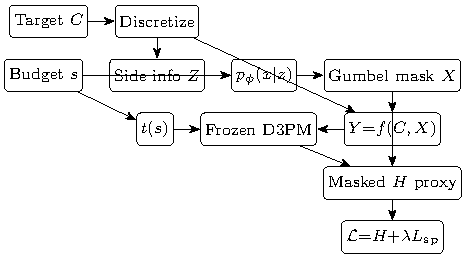
\includegraphics[width=\columnwidth]{figures/pipeline.pdf}
\caption{Training pipeline: mask generator $p_\phi(x \mid z)$ minimizes masked conditional-entropy proxy under a sparsity budget using a frozen D3PM prior.}
\label{fig:pipeline}
\end{figure}

\section{Experiments: MNIST and CIFAR-10}

\subsection{Setup}
\begin{table}[t]
\centering
\small
\begin{tabular}{lcc}
\hline
\textbf{Setting} & \textbf{MNIST} & \textbf{CIFAR-10} \\
\hline
Mask architecture & Spatial & Spatial \\
Batch size & 512 & 256 \\
Learning rate & $3 \times 10^{-4}$ & $2 \times 10^{-5}$ \\
$\lambda$ (sparsity) & 10.0 & 1.0 \\
Sparsity range & $[0.05, 0.95]$ & $[0.1, 0.9]$ \\
Gumbel $\tau$ & $1.0 \rightarrow 0.5$ & $1.0 \rightarrow 0.5$ \\
Epochs & 200 & 200 \\
\hline
\end{tabular}
\caption{Mask-generator training hyperparameters.}
\label{tab:hyper}
\end{table}

\subsection{Evaluation Protocol}
\texttt{itw/eval.py} compares learned masks against \textbf{random masks} with matched sparsity. Metrics include $\mathcal{H}_{\mathrm{learned}}$, $\mathcal{H}_{\mathrm{random}}$, $\Delta H = \mathcal{H}_{\mathrm{random}} - \mathcal{H}_{\mathrm{learned}}$ (higher is better), and sparsity error $|\bar{X} - s|$.

\subsection{Results}
\textbf{MNIST.} Training logs show consistent decrease in the entropy proxy (Table~\ref{tab:mnist-results}). The proxy drops roughly $4\times$ while sparsity loss remains below $10^{-3}$.

\begin{table}[t]
\centering
\small
\begin{tabular}{cccc}
\hline
\textbf{Epoch} & $\mathcal{H}_{\mathrm{proxy}}$ & $\mathcal{L}_{\mathrm{sparsity}}$ & $\tau$ \\
\hline
0 & 0.029 & 0.0008 & 1.00 \\
10 & 0.008 & 0.0002 & 0.97 \\
29 & 0.007 & 0.0003 & 0.93 \\
39 & 0.006 & 0.0002 & 0.90 \\
\hline
\end{tabular}
\caption{MNIST mask training (\texttt{itw/} pipeline).}
\label{tab:mnist-results}
\end{table}

\textbf{CIFAR-10 (pre-fix runs).} Earlier experiments \emph{without} masked-only entropy showed $\mathcal{H}_{\mathrm{proxy}}$ \textbf{increasing} over epochs despite falling sparsity loss---motivating the methodological fixes here. Re-training with \texttt{itw/} is required for valid CIFAR conclusions.

\subsection{Reproducibility}
MNIST and CIFAR workflows are in \texttt{20260415\_itw\_mnist.ipynb} and \texttt{20260416\_itw\_cifar10.ipynb}. Entry point: \texttt{from itw import MNISTConfig, train\_mask\_generator}.

\section{Accelerated MRI: a stress test}

MNIST and CIFAR-10 evaluate the proxy against itself: the quantity reported ($\mathcal{H}_{\mathrm{proxy}}$) is the quantity optimized. Accelerated MRI breaks that circularity. The action is a Cartesian phase-encode (PE) row mask under a line budget, and the mask can be scored by reconstruction error, which the policy never sees.

\subsection{Setup}
fastMRI single-coil \cite{zbontar2018fastmri}, one mid-slice per volume: 973 train and \textbf{199 held-out validation} files at $300 \times 300$. The action is a 300-row mask with a 32-row auto-calibration (ACS) block locked on; the budget is enforced exactly by top-$k$ selection, so every method compares at identical density. Side information $Z$ is a central scout reconstruction. We report per-slice $\mathrm{NMSE} = \lVert \hat{c} - c \rVert^2 / \lVert c \rVert^2$ averaged over slices; stochastic baselines are averaged over 5 seeds and a margin inside $2$ standard deviations is not counted as a win.

Two reconstructors are trained on the training split under \emph{heuristic} masks only, so neither ever sees a learned mask: \textbf{U-Net A}, against which masks are optimized, and \textbf{U-Net B}, an independently initialized \emph{judge} used only for scoring. All reported numbers are U-Net B.

\subsection{The proxy does not transfer}
\textbf{The entropy proxy disagrees with reconstruction quality.} At $s = 0.25$ the learned policy attains the lowest coarse proxy entropy $\mathcal{H}_c$ of any method and still loses on NMSE to every heuristic tested.

\textbf{A 300-number average beats the learned policy.} Mean per-row k-space energy, fit on the training split, beats the learned policy at every sparsity under zero-filled reconstruction ($+5.1\%$, $+0.5\%$, $+2.9\%$, $+3.6\%$ at $s = 0.25, 0.40, 0.50, 0.75$). The policy approximates that profile slightly worse: its row-selection frequency correlates $r = 0.93$ with the variable-density prior and $0.83$ with log row energy, with $77$--$81\%$ row overlap.

\textbf{Conditioning is barely used.} Replacing each slice's scout with \emph{another slice's} (a derangement with no fixed points) changes NMSE by $-0.35\%$ to $-0.80\%$ on average---the wrong scout is mildly \emph{better}. At $s = 0.25$ the correct scout does help ($+0.7\%$ under the judge), while at $s \geq 0.40$ conditioning is mildly harmful. The conditional architecture does not earn its complexity.

\subsection{Mask ranking is reconstructor-dependent}
The failure has a mechanism (Table~\ref{tab:recon-gain}). Masks that \textbf{spread out} gain most from a reconstructor; \textbf{center-concentrated} masks gain least. A reconstructor carrying a prior already predicts the low-frequency center, so budget spent there is redundant. The energy oracle---the best mask of all under zero-filled reconstruction---becomes the worst once a prior exists.

\begin{table}[t]
\centering
\small
\begin{tabular}{lccc}
\hline
\textbf{Mask} & \textbf{Zero-filled} & \textbf{U-Net B} & \textbf{Gain} \\
\hline
ACS + equispaced & 0.03820 & 0.02591 & 32.2\% \\
ACS + random & 0.03819 & 0.02661 & 30.3\% \\
ACS + variable density & 0.03382 & 0.02450 & 27.5\% \\
learned, static & 0.03470 & 0.02897 & 16.5\% \\
learned, adaptive & 0.03318 & 0.02785 & 16.1\% \\
energy oracle & 0.03147 & 0.02703 & 14.1\% \\
\hline
\end{tabular}
\caption{Val NMSE at $s = 0.25$. Center-concentrated masks gain least from a reconstructor that carries a prior.}
\label{tab:recon-gain}
\end{table}

This is why the information-theoretic policy underperforms: it was trained on zero-filled reconstruction error plus a coarse-entropy term, \textbf{both of which reward energy capture}, which is precisely the wrong signal once the reconstructor improves. The objective was not wrong about its own criterion; the criterion was the wrong one.

\subsection{What does work}
Optimizing the discrete mask directly against a reconstructor. Gradient-based relaxation (a straight-through top-$k$ over a 300-parameter row profile, in the spirit of \citet{bahadir2020loupe}) loses to variable density at every sparsity. A greedy row-swap search on the \emph{hard} mask---gradient proposes candidate swaps, exact evaluation accepts them, in the spirit of \citet{gozcu2018learning}---wins (Table~\ref{tab:mri-main}).

\begin{table}[t]
\centering
\small
\setlength{\tabcolsep}{4pt}
\begin{tabular}{lcccc}
\hline
$s$ & \textbf{Ours (static)} & \textbf{ACS + VD} & \textbf{Gain} & \textbf{LOUPE} \\
\hline
0.25 & \textbf{0.02355} & 0.02448 $\pm$ 0.00006 & $+3.79\%$ & 0.02698 \\
0.40 & \textbf{0.01842} & 0.01882 $\pm$ 0.00005 & $+2.14\%$ & 0.02245 \\
0.50 & \textbf{0.01521} & 0.01544 $\pm$ 0.00007 & $+1.49\%$ & 0.02024 \\
0.75 & 0.00763 & 0.00765 $\pm$ 0.00001 & $+0.18\%$ & 0.00974 \\
\hline
\end{tabular}
\caption{Held-out val NMSE under the judge U-Net B. ACS + VD: ACS block plus variable-density rows, 5 seeds. The first three gains over it exceed $2$ seed standard deviations; $s=0.75$ is a tie. LOUPE \citep{bahadir2020loupe}: row-restricted, trained to mask convergence, budget-exact top-$k$.}
\label{tab:mri-main}
\end{table}

It is the best mask tested on NMSE and PSNR at every sparsity, and it also beats variable density under plain zero-filled reconstruction at three of four sparsities, so it is not exploiting one reconstructor's quirks. SSIM agrees at $s \leq 0.50$ against variable density, but center-concentrated masks (the relaxed profile, the energy oracle) score up to $0.7$ SSIM points ($\times 100$) higher at $s \geq 0.40$.

We also ran LOUPE itself \citep{bahadir2020loupe} as a baseline, ported to PyTorch, restricted to whole phase-encode rows, trained to mask convergence on the same split, and made budget-exact by top-$k$. Its mask is $14.6$--$33.1\%$ worse than ours under the judge, and worse than every heuristic at $s \geq 0.40$, despite training its reconstructor jointly with the mask. LOUPE's forward model FFTs a real magnitude image, so its k-space is Hermitian. Its masks follow that assumption: at $s = 0.25$--$0.50$ they contain only $7$ mirrored $\pm f$ row pairs (ours: $19$--$57$), and at $s = 0.75$ they sample one full half of k-space. On true complex k-space the two halves are not redundant, which is the most plausible cause of the gap. We therefore read this as a limitation of LOUPE's forward model for complex data, not of relaxation as such. The gap between the relaxed and combinatorial optimizers is not small: the relaxed profile lost by $1.5$--$2.3\%$ where the discrete search won by $1.5$--$3.8\%$, on the same objective and data.

\subsection{Two controls worth adopting}
\textbf{The judge matters.} Scored against the reconstructor it was optimized against, the relaxed profile reads $-0.49\%$ versus variable density at $s = 0.40$; against an independently trained judge it reads $-1.97\%$. A full $1.5$ pp of apparent mask quality was overfitting to one reconstructor.

\textbf{A metric defect inverted two of our own conclusions.} Our NMSE implementation clamped the denominator $\lVert c \rVert^2$ at an absolute $10^{-8}$. FastMRI magnitude is $\sim 10^{-6}$, so $\lVert c \rVert^2 \approx 4.2 \times 10^{-9}$ for a median slice and the floor was active on $64\%$ of training and $67\%$ of validation slices, silently converting NMSE to a constant-scaled MSE on exactly the low-energy images and reading $\sim 4\times$ low. Correcting it reversed the sign of our scout-derangement result at $s = 0.25$ and removed a claimed win for the learned static mask. Every MRI number above is post-correction. We report this because the defect is invisible to any test that only checks relative ordering within one metric.

\section{Discussion and Limitations}

\textbf{MINE vs.\ D3PM proxy.} MINE requires a separate critic and can be unstable; the D3PM proxy reuses a generative prior, avoids adversarial estimation, and handles discrete states natively---at the cost of assuming the D3PM captures relevant uncertainty.

\textbf{Proxy validity.} $\mathcal{H}_{\mathrm{proxy}}$ is entropy of a frozen $c_0$-predictor, not rigorous $H(C \mid Y)$. The D3PM was trained on forward-noised inputs, not arbitrary mask patterns.

\textbf{Timestep alignment.} Matching $s$ to $t$ via pixel survival is heuristic; masked images are spatially structured whereas forward corruption is i.i.d.\ per pixel.

\textbf{Baselines.} Quantitative comparison to saliency or compression masks is not yet reported. Scope is \textbf{mask-only active acquisition}; coupling masks to D3PM reverse sampling is future work.

\textbf{The prior is not load-bearing in the MRI result.} This is the central limitation. The frozen D3PM contributes nothing to the winning MRI mask, which is produced by combinatorial search against a reconstructor. On MNIST the proxy decreases, but nothing independent of the proxy confirms the resulting masks are better; MRI is the one setting here with such an independent criterion, and there the proxy fails it. We therefore do not claim the D3PM surrogate is validated as an acquisition objective---only that it is optimizable, not that it is useful.

\textbf{Why the negative result may be specific.} The fine-resolution prior is flat in cross-entropy across timesteps, so it supplies no usable gradient and was disabled ($\beta = 0$) in all MRI runs; only the coarse row-profile prior is active. A stronger prior---or a diffusion posterior sampler as the reconstructor rather than a U-Net---could change the conclusion, and our own results show the optimal mask moves when the reconstructor does.

\textbf{Scale and local optimality.} Single-coil, one mid-slice per volume, 973 training images, and reconstructors of 1.9M/4.3M parameters. The combinatorial search stops when no single row swap among 24 gradient-proposed candidates improves; it is a local optimum, not a global one.

\section{Conclusion}

We presented an information-theoretic framework for active data acquisition with side information under resource constraints, extending prior MINE-based blind estimation to \textbf{discrete images} via a frozen D3PM conditional-entropy surrogate, combining masked-only entropy, sparsity--timestep calibration, and Gumbel-Softmax mask training. On MNIST the surrogate optimizes cleanly.

Tested on accelerated MRI---where masks can be scored by a criterion the policy never sees---the framework does not hold up in its conditional form. The proxy disagrees with reconstruction quality, per-slice conditioning is worth at most $2\%$, and a 300-number energy average outperforms the learned policy. The mechanism is that mask ranking is \textbf{reconstructor-dependent}: an objective built on zero-filled error and prior entropy rewards energy capture, which is exactly what a reconstructor with a prior makes redundant. Optimizing the discrete mask against the reconstructor instead yields a static mask that beats variable density by $1.5$--$3.8\%$ NMSE under a held-out judge.

We take two lessons to be more durable than the specific numbers. First, an acquisition objective must be trained against the estimator that will actually be used, because the optimal measurement set is a property of the pair, not of the signal alone. Second, a surrogate that decreases under its own optimization is not thereby validated; the MNIST and MRI results differ precisely in whether an independent criterion was available. We release \texttt{itw/} with the held-out protocol, the derangement and judge controls, and the reconstructor, so that both the positive and negative results here can be checked and contested.

\bibliography{references}

\end{document}
